\documentclass[oneside]{report}
\usepackage{graphicx}
\usepackage{xepersian}
\settextfont{XB Niloofar}
\title{
    
\includegraphics[width=0.5\linewidth]{3.png}
    \\
    پروژه ایریدیوم
}
\author{سایین اعلا \\ \and گلبرگ سپهرآرا}
\date{پاییز ۱۴۰۲}

\begin{document}

\maketitle

\subsection*{مقدمه}
در این پروژه هدف این است که یک دستگاه قربانی پیدا بکنیم و پس اتصال به دستگاه قربانی فایل bash  را اجرا کنیم که اطلاعاتی از سیستم قربانی بدهد.
\\
در این مرحله پروژه به چند فاز تقسیم که در فاز اول درباره attacker  است و در فاز دوم درباره نحوه اتصال و ساخت شبکه با استفاده از docker است گفته شده است

\subsection*{Attacker}
در قسمت attacker فایل bash.sh  وجود دارد که در ابتدا بررسی میکند با IP addres مربوطه کدام subnet  ها و  ip  ها reachable  هستند و از بین این ها کدام  port  ها باز هستند که در فایل outputfile  دخیره میشوند
(برای پیدا کردن port  های باز  از nmap استفاده شد)
\\
در فایل merge.py  هم دوفایل username  و  password .csv  را که لیستی از یوزرنیم و پسورد های ما است را خوانده
و تمامی حالات ممکن و قابل قبول را در فایل username-pass.csv  میریزد
\\
این برنامه یک اسکریپت Bash است که برای تست ورود به سیستم‌های مختلف با استفاده از یک فایل CSV حاوی اطلاعات ورود (نام کاربری و رمز عبور) و یک فایل CSV حاوی آدرس‌های IP استفاده می‌شود. هدف اصلی این برنامه تست ورود به سیستم با استفاده از ابزار sshpass است.

در ابتدا، متغیرهایی برای مسیر فایل CSV حاوی اطلاعات ورود (csv_file)، مسیر فایل خروجی برای نتایج ورود به سیستم (output_file) و مسیر فایل CSV حاوی آدرس‌های IP (IPs) تعریف می‌شوند.

سپس، با دستور echo، سربرگ CSV به فایل خروجی اضافه می‌شود. سپس با استفاده از دستور tail، خط اول (سربرگ) فایل IPs را صرف نظر می‌کنیم.

در حلقه اول while، آدرس‌های IP را خوانده و در متغیر ip ذخیره می‌کنیم. درون حلقه دوم while، نام کاربری و رمز عبور را خوانده و در متغیرهای username و password ذخیره می‌کنیم.

سپس، نام کاربری و رمز عبور را به فایل خروجی اضافه کرده و با استفاده از ابزار sshpass و دستور ssh، تلاش برای ورود به سیستم با اطلاعات ورود فعلی انجام می‌دهیم. اگر ورود موفقیت‌آمیز بود، وضعیت ورود را به "Success" تغییر می‌دهیم و نتیجه ورود را به فایل خروجی اضافه می‌کنیم. در صورت ورود موفقیت‌آمیز، حلقه while بیرونی نیز قطع می‌شود.

در صورتی که هیچ ورود موفقیت‌آمیزی در حلقه while داخلی یافت نشود، برنامه به حلقه while بیرونی برمی‌گردد و اجرای برنامه خاتمه می‌یابد.
\begin{center}
    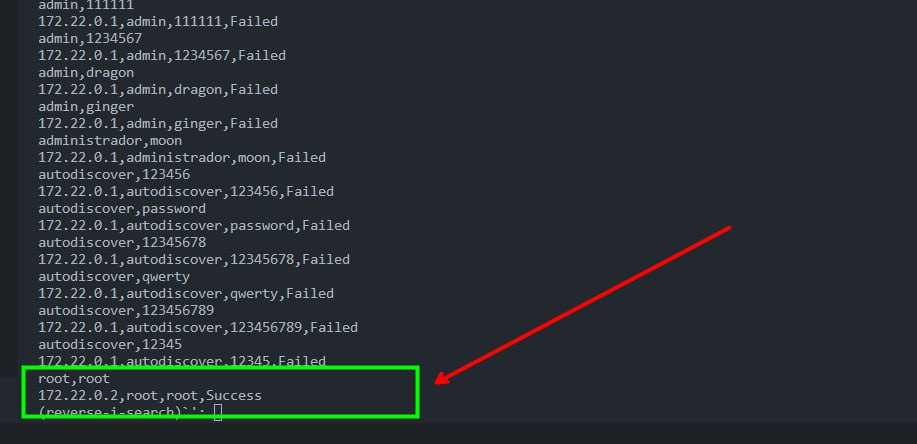
\includegraphics[height=0.5\linewidth]{finding_password.png}
\end{center}

\subsection*{Victim}
در نسخه قربانی ابتدا نیاز داریم یک شبکه داکر بسازیم
\\
این برنامه یک اسکریپت Bash است که برای محیط تست و شبیه‌سازی یک شبکه داخلی با استفاده از Docker استفاده می‌شود. در طول اجرای برنامه، شبکه داخلی ایجاد می‌شود و سرویس‌های مختلفی روی سرورهای هدف اجرا می‌شوند. همچنین یک سرور وب و یک ماشین حمله نیز ایجاد می‌شوند.

برنامه در ابتدا با استفاده از دستور echo، خطوط جداکننده برای بخش‌های مختلف برنامه چاپ می‌کند.

سپس با استفاده از دستور docker network create، یک شبکه با نام testnet ایجاد می‌شود.

بعد از آن، با استفاده از دستورات docker run، سه سرور هدف با نام‌های ser1، ser2 و ser3 ایجاد می‌شوند و به شبکه testnet متصل می‌شوند. این سرورها روی تصویری با نام target اجرا می‌شوند و در حالت پیش‌فرض با کاربر root اجرا می‌شوند.

سپس با استفاده از دستورات docker exec، سرویس‌های SSH، FTP و crond روی هر سرور هدف فعال می‌شوند.

در مرحله بعد، یک سرور وب با نام web ایجاد می‌شود که در بستر شبکه testnet قرار دارد و پورت 8000 را به پورت 8000 سیستم میزبان متصل می‌کند.

در نهایت، یک ماشین حمله با نام attacker ایجاد می‌شود که به شبکه testnet متصل می‌شود و در حالت تعاملی اجرا می‌شود.
\\
\begin{center}
    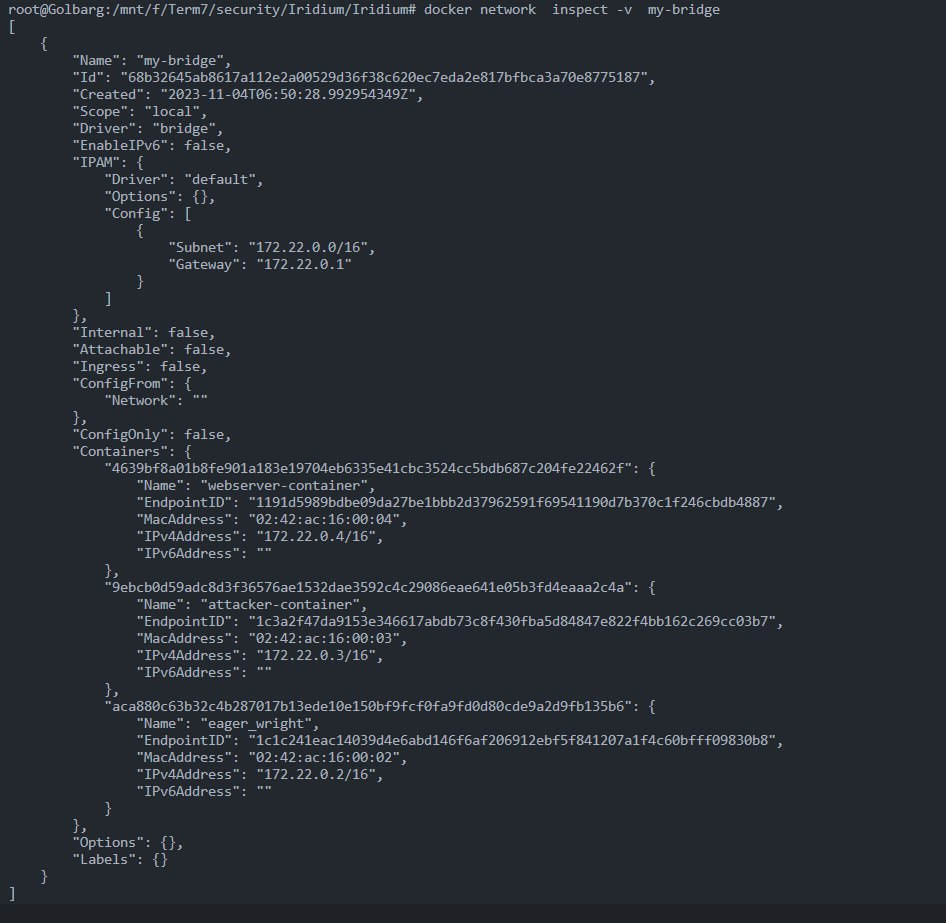
\includegraphics[height=0.5\linewidth]{1.png}
\end{center}
\\
این برنامه یک فایل Dockerfile است که برای ساخت یک تصویر Docker استفاده می‌شود. این تصویر بر اساس توزیع Alpine استوار است و برخی از بسته‌ها و تنظیمات مورد نیاز را نصب و پیکربندی می‌کند.

در ابتدا، از تصویر پایه Alpine:latest استفاده می‌شود. این تصویر حاوی جدیدترین نسخه از توزیع Alpine Linux است.

سپس، با استفاده از دستور USER، کاربر ریشه (root) تعیین می‌شود که برای اجرای دستورات بعدی استفاده می‌شود.

در دستور بعدی، با استفاده از دستور RUN و دستور passwd، رمز عبور برای کاربر root به "root" تنظیم می‌شود.

سپس، با استفاده از دستور RUN، بسته‌های مورد نیاز را نصب می‌کنیم. این شامل بروزرسانی بسته‌ها (apk update)، نصب بسته‌های busybox-extras، openssh، openssh-server، openrc، nmap، curl، sshpass و bash است.

در دستور بعدی، با استفاده از دستور echo، تنظیمات SSH را در فایل /etc/ssh/sshd_config اعمال می‌کنیم. اجازه ورود ریشه (PermitRootLogin) و احراز هویت با رمز عبور (PasswordAuthentication) فعال می‌شود. سپس با استفاده از دستور rc-status، وضعیت سرویس‌ها بررسی می‌شود و با استفاده از دستور touch، سطح نرم‌افزاری /run/openrc/softlevel تعیین می‌شود.

در دستور بعدی، بسته vsftpd نیز نصب می‌شود.

سپس، با استفاده از دستور rc-update، سرویس vsftpd به عنوان سرویس پیش‌فرض برای اجرا تنظیم می‌شود.

در دستور بعدی، با استفاده از دستور COPY، تمام فایل‌های موجود در مسیر فعلی (فایل‌های سورس) را به مسیر /root/ درون تصویر Docker منتقل می‌کنیم.

در نهایت، با استفاده از دستور CMD، فرآیند اصلی تعیین می‌شود که در اینجا یک شل Bash است و در داخل تصویر Docker اجرا خواهد شد.
\\
برنامه فوق یک فایل Dockerfile است که برای ساخت تصویر Docker استفاده می‌شود. این تصویر شامل سیستم عامل Alpine است که به عنوان پایه استفاده می‌شود و برخی از سرویس‌ها و ابزارهای دیگر نیز در آن نصب می‌شوند.

در ابتدا، کاربر ریشه (root) تعریف می‌شود و سپس سه پورت (22، 1234 و 5678) با استفاده از دستور EXPOSE اعلام می‌شوند. این پورت‌ها برای ارتباط با سرویس‌های دیگر استفاده خواهند شد.

سپس با استفاده از دستور RUN، دستورات لازم برای نصب بسته‌ها و تنظیمات سیستم اجرا می‌شوند. این شامل بروزرسانی بسته‌ها (apk update)، نصب بسته‌های busybox-extras، busybox-openrc، openssh، openssh-server، openrc، curl و bash است. همچنین تنظیماتی برای SSH اعمال می‌شود تا اجازه ورود ریشه (PermitRootLogin) و احراز هویت با رمز عبور (PasswordAuthentication) را فعال کند. در نهایت، سرویس‌ها و سطح نرم‌افزاری راه‌اندازی می‌شوند.

دستورات بعدی شامل نصب بسته vsftpd و اضافه کردن آن به لیست سرویس‌های راه‌اندازی به صورت پیش‌فرض است (rc-update add vsftpd default).

در نهایت، با استفاده از دستور CMD، پردازه /bin/bash به عنوان فرآیند اصلی برنامه تعریف می‌شود که به عنوان شل پیش فرض در داخل تصویر Docker اجرا خواهد شد.
محتوا کامل خروجی در فایل resault.txt  نمایش داده میشود.

\begin{center}
    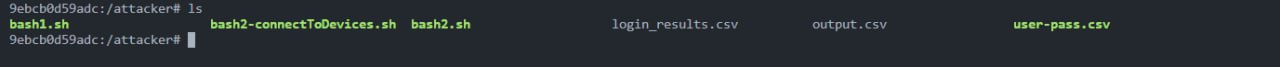
\includegraphics[width=1\linewidth]{attacker_container.png}
\end{center}

\\
در قسمت attacker  هم یک برنامه تحت وب توسط زده شده. django زده شده است که اطلاعات فرد در
در برنامه script.sh این برنامه یک اسکریپت Shell است که اطلاعات سیستم را جمع آوری کرده و در یک فایل JSON ذخیره می‌کند. سپس این فایل JSON را به یک آدرس وب ارسال می‌کند.

در ابتدا، مسیر فایل خروجی و نام فایل JSON تعیین می‌شود و یک فایل جدید باز می‌شود.

سپس با استفاده از دستورات echo و grep، نوع و نسخه لینوکس را از فایل /etc/os-release استخراج می‌کند و در فایل JSON ذخیره می‌کند.

در مرحله بعد، با استفاده از دستور cat، اطلاعات پردازنده را از فایل /proc/cpuinfo استخراج می‌کند و در فایل JSON ذخیره می‌کند.

سپس، با استفاده از دستور date، تاریخ و زمان سیستم را جمع آوری می‌کند و در فایل JSON ذخیره می‌کند.

در بخش بعدی، با استفاده از دستور df، اطلاعات فضای مصرف شده در دیسک‌ها را جمع آوری می‌کند و در فایل JSON ذخیره می‌کند.

در آخر، با استفاده از دستور curl، فایل JSON را به یک آدرس وب ارسال می‌کند. آدرس وب ورودی به عنوان پارامتر اول به اسکریپت داده می‌شود و فایل JSON به عنوان بدنه درخواست POST با استفاده از پوشه 'app/post-info/' در آدرس وب ارسال می‌شود.

برای ران کردن ssh  از این دستور استفاده شده است:
\begin{center}
    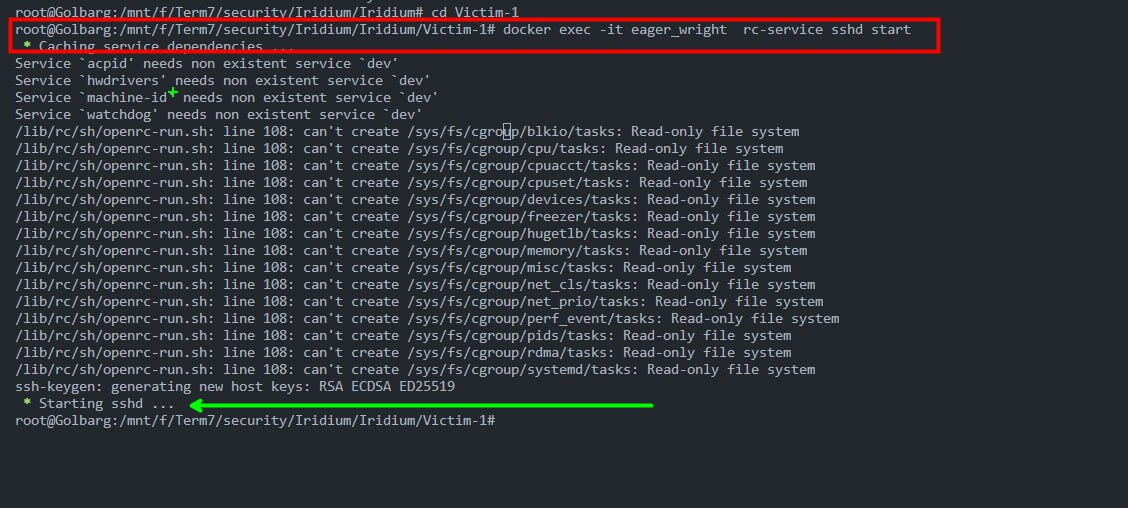
\includegraphics[height=0.5\linewidth]{run_ssh.png}
\end{center}
دیتا بیس :
\begin{center}
    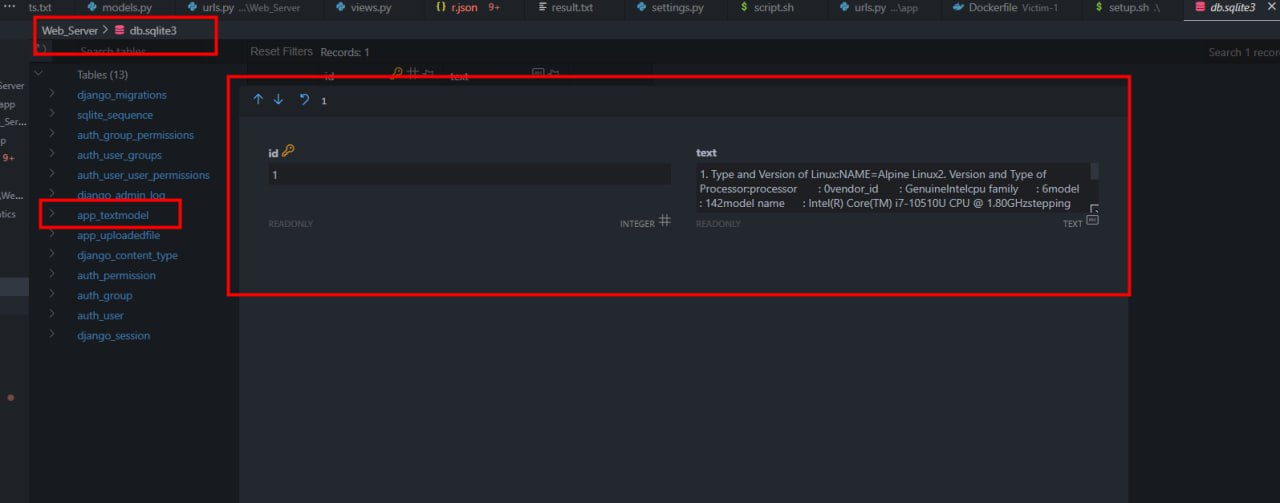
\includegraphics[height=0.5\linewidth]{database.png}
\end{center}


\end{document}
